\chapter{Der neue Ansatz} \label{der-neue-ansatz}

% Mehr Projekte nutzen TypeScript => sind bereits was Typing angeht robust
TypeScript wird von immer mehr Entwicklern genutzt, während die JavaScript Nutzung abnimmt. TypeScript verfügt im Gegensatz zu JavaScript über ein statisches Typisierungssystem. Diese Eigenschaft reduziert Fehler, die aufgrund von inkonsisten oder falschen Typen entstehen, erheblich.

% TypeScript ist auch in fast allen IDEs integriert, also wird fast von jedem genutzt.

\begin{figure}[h!]
  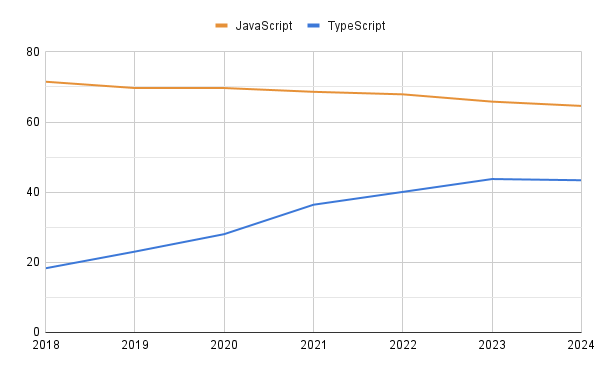
\includegraphics[width=1\textwidth]{js-und-ts-nutzung-2018-2024.png}
  \caption{Prozentuale Nutzung von JavaScript und TypeScript unter professionellen Entwicklern von 2018 bis 2024}
  \label{fig:js-und-ts-nutzung-2018-2024}
\end{figure}

% Um Implementierungsfehler zu vermeiden => Transitions robuster machen